\documentclass[a4paper, twocolumn]{article}
\usepackage[pdftex, hidelinks,
            pdftitle={Machine Learning Report},
            pdfauthor={Erik Sven Vasconcelos Jansson},
            pdfsubject={Machine Learning Report},
            pdfkeywords={report}]{hyperref}

\usepackage{bm}
\usepackage[T1]{fontenc}
\usepackage[utf8]{inputenc}
\usepackage{algorithmic}
\usepackage{algorithm}
\usepackage{amsfonts}
\usepackage{booktabs}
\usepackage{amssymb}
\usepackage{courier}
\usepackage{booktabs}
\usepackage{graphicx}
\usepackage{listings}
\usepackage{mathtools}
\usepackage[capitalize, noabbrev]{cleveref}
\lstset{basicstyle=\footnotesize\ttfamily,
        breakatwhitespace = false,
        breaklines = true,
        keepspaces = true,
        language = R,
        showspaces = false,
        showstringspaces = false,
        belowcaptionskip = \bigskipamount,
        framerule = 0.80pt,
        frame = tb,
        numbers = left,
        belowskip = \bigskipamount,
        escapeinside={<@}{@>}}

\title{Introduction to Machine Learning \\
       Individual Laboration Report --5--}
\author{{Erik Sven Vasconcelos Jansson} \\
        {\href{mailto:erija578@student.liu.se}
        {\texttt{erija578@student.liu.se}}} \\
        {Linköping University, \, Sweden}}

\begin{document}

    \pagenumbering{arabic}
    \maketitle % Titles...

    Increasing the accuracy of \emph{weather forecasts} is an important task. We propose an estimator which produces the \emph{air temperature forecast} in \emph{Sweden}, given a \emph{latitude/longitude coordinate} and also \emph{date}. Some observations by \emph{SMHI}, taken from weather stations, have been given for training our estimator.

    By using a \emph{Nadaraya–Watson regression kernel}, we can estimate the temperatures \(\bm{y'}\). This is done by taking the \emph{kernels} \(k_\sigma(\bm{x}^{(i)}, \bm{x'})\) for each \(i^{th}\) data from the training set and using it as a \emph{weight} when considering the response variable \(\bm{y}^{(i)}\). Essentially, the kernel \(k_\sigma(\bm{x}^{(i)}, \bm{x'})\) will reduce \(\bm{y}^{(i)}\)'s significance in the \emph{total contribution} by giving less weight when the \(\bm{x^{(i)}}\) and \(\bm{x'}\) are further away (in some measure).

    We have used a \emph{Gaussian Radial Basis Function} as our \emph{kernel}, which is defined in Equation~\ref{eq:grbf} below. Note the parameter \(\sigma\), which can be considered as the \emph{spread} or \emph{width} of the kernel, and also \(\bm{x^{(i)}} - \bm{x'}\) which is the \emph{distance function}; giving our kernel the property of a \emph{similarity function} (because of \(e^{(\cdots)}\)).

    By using \(k_\sigma(\bm{x}^{(i)}, \bm{x'})\) in \emph{Nadaraya–Watson's} \(\bm{y'}\) estimator, shown in Equation~\ref{eq:nadaraya_watson}, we are essentially \emph{weighing} how important the contributions from \(\bm{y}^{(i)}\) are to \(\bm{y'}\), because \emph{similar} \(\bm{x}^{(i)}\) will give higher \(k_\sigma\).

    \begin{equation} \label{eq:grbf}
        k_\sigma(\bm{x}, \bm{x'}) = \mathrm{exp}\bigg(\frac{- \, {\left\Vert(\bm{x} - \bm{x'}) \right\Vert}^2}
                                                           {2\sigma^2 \; \{\sigma \approx h\}}\bigg)
    \end{equation}

    \begin{equation} \label{eq:nadaraya_watson}
        \bm{y'}(\bm{x}, \bm{x'}) = \frac{\sum_n{\bm{y}^{(i)}k_\sigma(\bm{x}^{(i)}, \bm{x'})}}
                                               {\sum_n{k_\sigma(\bm{x}^{(i)}, \bm{x'})}}
    \end{equation}

    Practically, the \emph{kernel} is calculated in Listing~\ref{lst:forecast} under \texttt{gaussian\_kernel} and the \emph{estimation} is being done in the function \texttt{forecast}. However, note that the final contributions use \texttt{forecast\_kernel}, which will be described now.

    Below follows the applied \emph{distance functions}, which give the measured distance between a pair of \emph{locations}, \emph{times of the day}, and also \emph{dates of year}. These are used in \texttt{forecast\_kernel} for each respective \texttt{gaussian\_kernel} invocation. Additionally, these distances are \emph{normalized} to range in-between 0.0 - 1.0. See Listing~\ref{lst:forecast} for these values.

    \begin{equation*} \label{eq:location}
        d_l = r\, \mathrm{hav}^{-1}(h),\; \mathrm{hav}(\varphi) = \frac{1 - \cos\varphi}{2}
    \end{equation*}

    \begin{equation*} \label{eq:time}
        d_t = \begin{cases}
            |x - y| & |x - y| < (x + y) \bmod 24\\
            (x + y) \bmod 24 & |x - y| \geq (x + y) \bmod 24
        \end{cases}
    \end{equation*}

    \begin{equation*} \label{eq:day}
        d_d = \begin{cases}
            |x - y| & |x - y| < (x + y) \bmod 365\\
            (x + y) \bmod 24 & |x - y| \geq (x + y) \bmod 365
        \end{cases}
    \end{equation*}

    Therefore, the final \texttt{forecast\_kernel} is being calculated as seen below, where $k_l$ uses the \emph{location distance}, $k_d$ the \emph{date distance} and $k_t$ \emph{time distance}.

    \begin{equation*} \label{eq:forecast}
        k_f(\bm{x}, \bm{x'}) = k_l(\bm{x}, \bm{x'}) + k_d(\bm{x}, \bm{x'}) + k_t(\bm{x}, \bm{x'})
    \end{equation*}

    Within Table~\ref{tab:spread} are our chosen $\sigma$/$h$ \emph{spread}/\emph{width}.

    \begin{table}[h!]
        \begin{center}
            \begin{tabular}{lc}
                \toprule
                \textbf{Feature} & \textbf{Spread}\\
                \midrule
                Location & \(0.192\) \\
                Day &      \(0.256\) \\
                Time &     \(0.256\) \\
                \bottomrule
            \end{tabular}
        \end{center}
        \caption{Kernel Width}
        \label{tab:spread}
    \end{table}

    These have been chosen to decrease contribution, so for example \emph{locations} are not easily influenced...

    \clearpage

    Finally, we estimate $\bm{y}$ for \emph{2013-10-04} during the entire day in \emph{58.4274 latitude} and \emph{14.826 longitude}. See Table~\ref{tab:forecast} and Figure~\ref{fig:forecast} for the predicted results.

    \begin{table}[h!]
        \begin{center}
            \begin{tabular}{lc}
                \toprule
                \textbf{Time} & \textbf{Temperature ($^\circ$C)} \\
                \midrule
                04:00 & 4.478177 \\
                06:00 & 4.614255 \\
                08:00 & 4.846348 \\
                10:00 & 5.097822 \\
                12:00 & 5.256865 \\
                14:00 & 5.264849 \\
                16:00 & 5.149687 \\
                18:00 & 4.978578 \\
                20:00 & 4.799737 \\
                22:00 & 4.637349 \\
                24:00 & 4.512750 \\
                \bottomrule
            \end{tabular}
        \end{center}
        \caption{Forecast for 2013-11-04}
        \label{tab:forecast}
    \end{table}

    \begin{figure}[h!]
        \centering
        \caption{Air Temperature Forecast Graphs}
        \label{fig:forecast}
        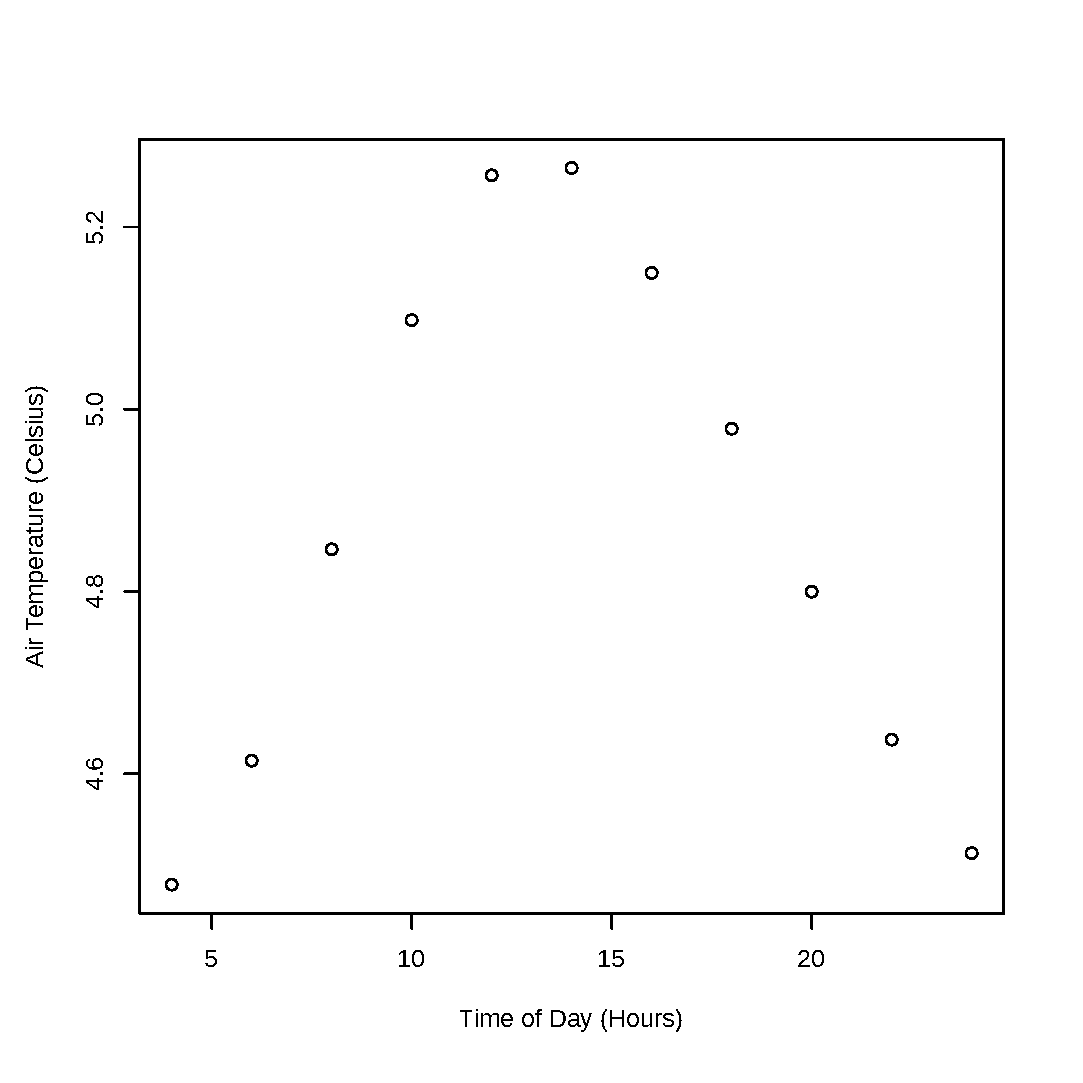
\includegraphics[width=0.5\textwidth]{share/forecast.eps}
    \end{figure}

    Notice how the plot above produces a \emph{bell curve}, which is to be expected from a temperature forecast according to previous data given by \emph{SMHI}. Also, these values don't seem to be that far off the truth, however they seem to be slightly colder than usual. One possible cause for this can be motivated by the \emph{independence} of each \emph{kernel}, outweighing the other.

    For example, assume both \emph{location} and \emph{time of day} are highly correlated to our $\bm{x'}$, therefore, they will \emph{contribute highly} with their $\bm{y^{(i)}}$. Now, for the sake of argument, assume \emph{day of the year} is \emph{not highly correlated} with $\bm{x'}$, therefore, the contribution $\bm{y^{(i)}}$ will not be significant, at least not compared to \emph{location} and \emph{time of day}. Therefore, even if we are taking an observation which is far away from the requested date, the contribution will still be high, which leads to most predictions being influenced with the ``mean'' temperatures in Sweden. Therefore, our hypothesis why most predictions are colder than expected is because the three kernels are being accounted independently of each other...

    Additionally, some words need to be said regarding our choice for the \emph{kernel spread/width} values in Table~\ref{tab:spread}. These were chosen on the assumption that \emph{locations} further away than \emph{350 kilometers} are not very good contributors, as are \emph{dates} with a distance further away than \emph{45 days} and between \emph{$\approx$5 hours}. The $\sigma$ where chosen such that these values were reached, and only correlated less than $10 \%$, thereafter proceeding with normal Gaussian falloff.

    \nocite{*}
    \bibliographystyle{alpha}
    \bibliography{report}

    \onecolumn \appendix
    \section*{Appendix}

    \lstinputlisting[caption={Nadaraya–Watson Gaussian Radial Basis Function Kernel Forecast Estimator},label={lst:forecast}]{../forecast.r}

\end{document}
